% =====================================================================
%  Relazione progetto di Fondamenti di Automatica - Traccia 28
%  Bruni Christian, matricola 240008
%
%  Riscrittura in LaTeX della relazione originale. La prosa e la
%  matematica sono ri-tipografate nativamente; i grafici e gli output
%  simbolici di Mathematica/Simulink sono le immagini estratte dal PDF
%  originale (cartella img/), non riproducibili senza i software.
%
%  Compilazione:  latexmk -pdf main.tex      (oppure pdflatex main.tex x2)
% =====================================================================
\documentclass[11pt,a4paper]{article}

\usepackage[utf8]{inputenc}
\usepackage[T1]{fontenc}
\usepackage[italian]{babel}
\usepackage{lmodern}
\usepackage{amsmath,amssymb,mathtools}
\usepackage{graphicx}
\usepackage{float}
\usepackage[font=small,labelformat=empty]{caption}
\usepackage[margin=2.5cm]{geometry}
\usepackage{xcolor}
\usepackage{enumitem}
\usepackage{hyperref}
\hypersetup{hidelinks}

\graphicspath{{img/}}

% --- helper per le immagini estratte dal PDF originale ---
% grafico/output Mathematica senza didascalia
\newcommand{\mma}[2][0.7]{%
  \begin{figure}[H]\centering\includegraphics[width=#1\linewidth]{#2}\end{figure}}
% grafico con didascalia (riprende le didascalie della relazione originale)
\newcommand{\mmacap}[3][0.7]{%
  \begin{figure}[H]\centering\includegraphics[width=#1\linewidth]{#2}\caption*{\itshape #3}\end{figure}}

\newcommand{\Lapl}{\mathcal{L}}
\newcommand{\Ztr}{\mathcal{Z}}

\title{\vspace{-1.5cm}\textbf{Relazione progetto\\Fondamenti di Automatica}}
\author{Bruni Christian \quad--\quad matricola 240008\\[2pt]Traccia n\textordmasculine\ 28}
\date{}

\begin{document}
\maketitle
\thispagestyle{empty}
\vspace{1cm}
\tableofcontents
\newpage

\section{Esercizio A -- Sistema LTI a tempo continuo}

Un sistema dinamico $\Sigma=(T,X,U,Y,\mathcal{U},\mathcal{Y},\phi,\eta)$ è una
collezione di insiemi, spazi e funzioni: $T$ è l'insieme dei tempi, $X$ lo spazio
di stato, $U$ e $Y$ le immagini di ingresso e uscita, $\mathcal{U}$ e $\mathcal{Y}$
gli insiemi delle funzioni di ingresso e di uscita ammissibili, $\phi$ la funzione
di transizione di stato (forma esplicita del sistema) ed $\eta$ la mappa di uscita.

Il sistema in esame è SISO (Single-Input Single-Output): ingresso e uscita sono
scalari. È inoltre \emph{proprio}, poiché la matrice $D$ è identicamente nulla e
quindi l'ingresso non influenza istantaneamente l'uscita. Le matrici sono:
\[
A=\begin{bmatrix}
-\tfrac{179}{4} & -\tfrac{331}{4} & \tfrac{205}{8} & -\tfrac{409}{8}\\[2pt]
\tfrac{183}{4} & \tfrac{327}{4} & -\tfrac{213}{8} & \tfrac{409}{8}\\[2pt]
-\tfrac{179}{2} & -\tfrac{331}{2} & \tfrac{205}{4} & -\tfrac{413}{4}\\[2pt]
-\tfrac{179}{2} & -\tfrac{327}{2} & \tfrac{209}{4} & -\tfrac{409}{4}
\end{bmatrix},\quad
B=\begin{bmatrix}-\tfrac12\\[2pt]\tfrac12\\[2pt]-1\\[2pt]-1\end{bmatrix},\quad
C=\begin{bmatrix}-10 & 0 & 0 & 5\end{bmatrix}.
\]

\subsection{Modi naturali}
I modi naturali sono funzioni reali di variabile reale che descrivono l'andamento
della risposta libera; si presentano nella forma $e^{\lambda_i t}$, con $\lambda_i$
l'$i$-esimo autovalore della matrice dinamica $A$. Gli autovalori sono
\[
\lambda_1=-7,\qquad \lambda_2=-3,\qquad \lambda_{3,4}=-2\pm\tfrac{j}{2}.
\]
Due reali e distinti, due complessi coniugati. Per ogni autovalore la molteplicità
algebrica coincide con la geometrica, quindi $A$ è diagonalizzabile. I modi associati
agli autovalori reali sono $e^{-7t}$ ed $e^{-3t}$; quelli legati alla coppia complessa
hanno forma $e^{\sigma t}\cos(\omega t)$ ed $e^{\sigma t}\sin(\omega t)$ con
$\sigma=\operatorname{Re}[\lambda]$ e $\omega=\operatorname{Im}[\lambda]$, cioè
$e^{-2t}\cos\!\big(\tfrac{t}{2}\big)$ ed $e^{-2t}\sin\!\big(-\tfrac{t}{2}\big)$.

\mmacap{img-003}{Andamento del 1\textordmasculine\ modo naturale}
\mmacap{img-004}{Andamento del 2\textordmasculine\ modo naturale}
\mmacap{img-005}{Andamento del 3\textordmasculine\ modo naturale}
\mmacap{img-006}{Andamento del 4\textordmasculine\ modo naturale}

\subsection{Risposta libera}
La risposta libera si ottiene da uno stato iniziale assegnato $x_0$ con ingresso
identicamente nullo, ed è una combinazione lineare dei modi naturali. Sullo stato vale
$x_l(t)=e^{At}x_0$; conviene diagonalizzare $A$ tramite una matrice di cambiamento di
base $T$ tale che $\Lambda=T^{-1}AT$, da cui $x_l(t)=T\,e^{\Lambda t}z_0$ con
$z_0=T^{-1}x_0$.

Per la coppia di autovalori complessi coniugati si costruisce una matrice $T$
``ibrida'', usando parte reale e immaginaria di un autovettore: in questo modo $T$
resta reale e $\Lambda$ assume la forma canonica reale con un blocco di Jordan
$2\times2$.

\mma[0.5]{img-013}

Si proietta lo stato iniziale $x_0=\begin{bmatrix}-1&0&-3&0\end{bmatrix}^{\!\top}$ sulle
colonne di $T$ ottenendo $z_0=T^{-1}x_0$; quindi la risposta libera sullo stato si
calcola come $x_l(t)=T\,\mathrm{MatrixExp}[\Lambda t]\,z_0$ e quella sull'uscita come
$y_l(t)=C\,x_l(t)$.

\mmacap{img-016}{Risposta libera sull'uscita confrontata con quella sullo stato}

\subsection{Configurazione degli stati iniziali}
Poiché la risposta libera è combinazione lineare dei modi naturali, una scelta
opportuna di $x_0$ può ``accendere'' o ``spegnere'' determinati modi. Scegliendo $x_0$
come combinazione lineare delle sole colonne di $T$ associate ai modi che si vogliono
evidenziare, le restanti componenti di $z_0$ si annullano e quei modi non compaiono.

\mmacap{img-018}{Accensione dei modi legati alle prime due colonne di $T$}
\mmacap{img-020}{Accensione dei modi legati alle ultime due colonne di $T$}
\mmacap[0.48]{img-021}{Solo prima colonna}
\mmacap[0.48]{img-022}{Solo seconda colonna}
\mmacap[0.48]{img-023}{Solo terza colonna}
\mmacap[0.48]{img-024}{Solo quarta colonna}

\subsection{Funzione di trasferimento, poli e zeri}
La funzione di trasferimento è la funzione di variabile complessa $G(s)$ tale che
$Y(s)=G(s)U(s)$, calcolata come $G(s)=C(sI-A)^{-1}B+D$ (qui $D=0$). Normalizzando
numeratore e denominatore rispetto al coefficiente di grado massimo si ottiene un
denominatore
\[
d(s)=s^4+14s^3+\tfrac{261}{4}s^2+\tfrac{253}{2}s+\tfrac{357}{4}.
\]

\mma[0.65]{img-025}

La correttezza si verifica con \texttt{StateSpaceModel}, che restituisce la forma di
Rosenbrock del sistema. I \emph{poli} sono le radici del denominatore (sempre un
sottoinsieme dei modi naturali); qui coincidono con gli autovalori:
\[
s=-7,\quad s=-3,\quad s=-2\pm\tfrac{j}{2}.
\]
Poiché i poli coincidono con gli autovalori, nella risposta forzata compaiono tutti i
modi naturali. Gli \emph{zeri} sono le radici del numeratore.

\subsection{Risposta al gradino unitario}
La risposta forzata al gradino è $Y(s)=G(s)\,U(s)$ con $\Lapl[1(t)]=\tfrac1s$.
Scomponendo $Y(s)$ in fratti semplici, la componente legata al polo $s=0$ è la
\emph{risposta a regime}, mentre quelle legate ai poli del sistema costituiscono la
\emph{risposta transitoria}. I residui si calcolano con la formula di Heaviside
\[
C_{ij}=\frac{1}{(v_i-j)!}\lim_{s\to p_i}\Big[(s-p_i)^{v_i}F(s)\Big].
\]
Per la coppia complessa è sufficiente calcolare $C_4$: $C_5=\overline{C_4}$.

\mmacap[0.85]{img-036}{Risposta forzata al gradino con le componenti $y_{ss}(t)$ e $y_{tr}(t)$}

\subsection{Risposta al segnale periodico elementare}
Si considera $u(t)=A\sin(\omega t+\psi)\,1(t)$ con la terna $A=2,\ \omega=2,\ \psi=0$.
Costruite $U(s)$ e $Y(s)$, si scompone in fratti semplici e, con la formula di
Heaviside, si separano la componente di regime (legata all'ingresso) e quella
transitoria (legata ai modi).

\mmacap[0.7]{img-038}{Risposta forzata al segnale sinusoidale e sue componenti}

Il sistema distorce il segnale in ampiezza e fase. Per quantificare i fattori di
distorsione si usa la forma \emph{amplitude-phase} $X\sin(\omega t+\psi)$, eguagliata
alla componente di regime nell'ipotesi di ingresso $\sin(t)\,1(t)$; dei fratti semplici
interessano solo quelli legati all'ingresso.

\mmacap[0.7]{img-050}{Confronto fra ingresso e componente di regime (forma amplitude-phase)}

Risolvendo si trova $X<1$: il segnale è attenuato in ampiezza e mostra un anticipo di
fase.

\subsection{Modello ARMA equivalente e risposta alla rampa}
Il modello ARMA (Auto-Regressive Moving Average) è una rappresentazione implicita
ingresso/uscita, un'equazione differenziale della forma
\[
y^{(n)}+a_1y^{(n-1)}+\dots+a_ny=b_0u^{(n)}+b_1u^{(n-1)}+\dots+b_nu,
\]
ricavabile da $G(s)=\tfrac{Y(s)}{U(s)}$. Le condizioni iniziali sull'uscita compatibili
con $x_0=\begin{bmatrix}-3&2&-3&3\end{bmatrix}^{\!\top}$ si ottengono dalla matrice di
osservabilità: $[\,y(0)\ \dot y(0)\ \ddot y(0)\ \dddot y(0)\,]^{\top}=\mathrm{Ob}\,x_0$,
con $\mathrm{Ob}=[\,C;\,CA;\,CA^2;\,CA^3\,]$. Per il sistema in esame:
\[
\dddot{\!\!\;y}^{\,(4)}+14\,\dddot y+\tfrac{261}{4}\ddot y+\tfrac{253}{2}\dot y+\tfrac{357}{4}y
=5\,\dot u-5\,u.
\]

\mma[0.85]{img-052}

Antitrasformando e confrontando la risposta libera ottenuta dal modello I/U con quella
ricavata dalla definizione I/S/U si verifica che le due coincidono, a conferma della
correttezza dei calcoli.

\paragraph{Risposta alla rampa unitaria.}
Con $\Lapl[t\,1(t)]=\tfrac{1}{s^2}$, si sostituiscono nel modello ARMA le condizioni
iniziali e la trasformata dell'ingresso, separando la componente transitoria (risposta
libera inclusa) da quella legata algebricamente all'ingresso:
\[
y_{ss}(t)=\frac{17260}{127449}-\frac{20\,t}{357}.
\]

\subsection{Stato iniziale che annulla il transitorio}
Si cerca $x_0$ tale che la risposta al gradino coincida con il suo valore di regime
(assenza di transitorio): occorre che la somma di risposta libera e risposta transitoria
sia identicamente nulla. Imponendo l'annullamento del numeratore (polinomio di terzo
grado nelle quattro incognite $x_i$) si ottiene
\[
x_0=\begin{bmatrix}\tfrac{2}{357}&-\tfrac{2}{357}&\tfrac{4}{357}&0\end{bmatrix}^{\!\top}.
\]
La verifica con \texttt{OutputResponse} applicato alla forma di Rosenbrock e il
confronto con $\mathrm{FdT}[0]$ danno valori coincidenti.

\subsection{Risposta al segnale $u(t)=1(-t)$}
L'ingresso $1(-t)$ vale $1$ per $t<0$ e $0$ per $t\ge0$. Lo si interpreta come un segnale
applicato in un passato remoto ($t\to-\infty$): la componente transitoria si è già
estinta e per $t<0$ resta solo la componente di regime. Per $t\ge0$ l'ingresso è nullo e
il sistema evolve liberamente a partire dalle condizioni all'istante $t=0$, ricavate da
$x_0=\mathrm{Ob}^{-1}\cdot\text{(condizioni iniziali)}$. La risposta complessiva si
descrive con un costrutto \texttt{Piecewise}.

\mmacap[0.55]{img-080}{Risposta del sistema all'ingresso $u(t)=1(-t)$}

\newpage
\section{Esercizio B -- Sistema LTI a tempo discreto}

Il sistema è $x(k+1)=Ax(k)+Bu(k)$, $y(k)=Cx(k)$, SISO e proprio, con
\[
A=\begin{bmatrix}
-\tfrac{92}{125} & -\tfrac{107}{125} & -\tfrac{43}{50}\\[2pt]
\tfrac{217}{125} & -\tfrac{18}{125} & -\tfrac{7}{50}\\[2pt]
-\tfrac{184}{125} & \tfrac{36}{125} & \tfrac{7}{25}
\end{bmatrix},\quad
B=\begin{bmatrix}-\tfrac12\\[2pt]\tfrac12\\[2pt]-1\end{bmatrix},\quad
C=\begin{bmatrix}\tfrac94 & -\tfrac74 & -2\end{bmatrix}.
\]

\subsection{Modi naturali}
Nei sistemi a tempo discreto i modi naturali sono successioni reali nella forma
$\lambda_i^{\,k}$. La matrice $A$ ha l'unico autovalore $\lambda=-\tfrac15$ con
molteplicità algebrica $3$ ma geometrica $1$: $A$ \emph{non} è diagonalizzabile.
\texttt{JordanDecomposition} restituisce la matrice di cambio base $T$ e la forma
canonica $\Lambda$ con un solo blocco di Jordan $3\times3$. I tre autovalori
coincidenti generano modi di tipo binomiale, secondo
\[
\sum_{i=0}^{l-1}\binom{k}{i}\lambda^{\,k-i},
\]
cioè $\lambda^k$, $\binom{k}{1}\lambda^{k-1}$ e $\binom{k}{2}\lambda^{k-2}$.

\mmacap[0.48]{img-084}{1\textordmasculine\ modo: $(-\tfrac15)^k$}
\mmacap[0.48]{img-085}{2\textordmasculine\ modo: $\binom{k}{1}(-\tfrac15)^{k-1}$}
\mmacap[0.48]{img-086}{3\textordmasculine\ modo: $\binom{k}{2}(-\tfrac15)^{k-2}$}

\subsection{Risposta libera}
La risposta libera sullo stato è $x(k)=A^k x_0$. Analogamente al caso continuo si cerca
una matrice simile ad $A$ tramite $T$: con $\mathrm{MatrixPower}[\Lambda,k]$ si ottiene
una matrice con, sulla diagonale, le potenze $k$-esime dei modi e, sulla triangolare
superiore, le successioni polinomio-potenza. Quindi $x_l(k)=T\,\Lambda^k z_0$ con
$z_0=T^{-1}x_0$, e $y_l(k)=C\,x_l(k)$. Lo stato iniziale è
$x_0=\begin{bmatrix}0&0&-3\end{bmatrix}^{\!\top}$.

\mmacap[0.48]{img-091}{Risposta libera sull'uscita $y_l[k]$}
\mmacap[0.48]{img-092}{Risposta libera sullo stato e sull'uscita a confronto}

\subsection{Attivazione di specifici modi naturali}
Come nel caso continuo, scegliendo opportune combinazioni lineari delle colonne di $T$
si attivano sulla risposta libera soltanto i modi desiderati.

\mmacap[0.48]{img-094}{Modi legati alle ultime due colonne di $T$}
\mmacap[0.48]{img-096}{Modi legati alla prima e all'ultima colonna}
\mmacap[0.48]{img-098}{Solo prima colonna}
\mmacap[0.48]{img-100}{Solo seconda colonna}
\mmacap[0.5]{img-102}{Solo terza colonna}

\subsection{Funzione di trasferimento, poli e zeri}
La funzione di trasferimento è ora funzione della variabile complessa $z$:
$Y(z)=G(z)U(z)$ con $G(z)=C(zI-A)^{-1}B+D$. Calcolata dalla definizione e normalizzata,
coincide con quella prodotta da \texttt{StateSpaceModel}. I poli sono le radici del
denominatore e, come sempre, sono un sottoinsieme degli autovalori: qui il polo triplo
$z=-\tfrac15$. Lo zero (radice del numeratore) è $z=-\tfrac18$.

\subsection{Risposta al gradino unitario}
La risposta forzata al gradino è $Y_f(z)=G(z)\,U(z)$ con $\Ztr[1(k)]=\tfrac{z}{z-1}$.
Si divide $Y_f(z)$ per $z$ per operare come nel tempo continuo e si scrivono i fratti
semplici. Per il residuo legato al polo $z=1$ (componente di regime) basta la formula di
Heaviside semplificata; per il polo triplo $z=-\tfrac15$ occorre quella generalizzata,
con le derivate successive
\[
C_{2j}=\frac{1}{(3-j)!}\lim_{z\to-\frac15}\frac{d^{\,3-j}}{dz^{\,3-j}}
\Big[(z+\tfrac15)^3\tfrac{Y_f(z)}{z}\Big].
\]
Antitrasformando (i modi binomiali danno i termini $\binom{k}{j}(-\tfrac15)^{k-j}$) si
ottiene la risposta come somma di componente di regime e transitoria.

\mmacap[0.7]{img-115}{Risposta al gradino con componenti $y_f[k]$, $y_{ss}[k]$, $y_{tr}[k]$}

Si verifica che la differenza poli$-$zeri (pari a $2$) è rispettata.

\subsection{Modello ARMA}
Partendo da $G(z)=\tfrac{Y(z)}{U(z)}$ e dalla matrice di osservabilità si ricavano le
condizioni iniziali sull'uscita compatibili con
$x_0=\begin{bmatrix}0&-2&-3\end{bmatrix}^{\!\top}$. Uguagliando
$\mathrm{den}(G)\,Y(z)=\mathrm{num}(G)\,U(z)$ e antitrasformando $z^nY(z)\to y(k+n)$ si
ottiene l'equazione alle differenze; nel dominio $z$ si calcola la risposta del sistema
e se ne isola la componente di risposta libera.

\mma[0.85]{img-122}

Confrontando la risposta libera dal modello ARMA con quella dalla definizione si verifica
l'uguaglianza, a conferma della correttezza delle condizioni iniziali e quindi
dell'equivalenza delle due rappresentazioni.

\paragraph{Risposta all'ingresso a finestra.}
L'ingresso vale $1$ per $0\le k\le10$ e $0$ altrove. Essendo di durata finita, la sua
trasformata $\Ztr$ si scrive come somma di potenze $\sum_{k=0}^{10}z^{-k}$.
Sostituendo questa trasformata e le condizioni iniziali nel modello I/U e
antitrasformando si ottiene la risposta del sistema.

\mmacap[0.48]{img-130}{Risposta totale all'ingresso a finestra}
\mmacap[0.48]{img-132}{Componente di regime della risposta}

\subsection{Condizioni iniziali ARMA che annullano il transitorio}
Con lo stesso ragionamento del caso continuo, si cercano le condizioni iniziali sull'uscita
tali che risposta libera $+$ transitoria sia identicamente nulla. Imponendo l'annullamento
dei coefficienti del numeratore (comandi \texttt{Solve} e \texttt{CoefficientList}) si
ottiene $y_0$, e da questo lo stato iniziale $x_0=\mathrm{Ob}^{-1}y_0$ con
$y_0=\begin{bmatrix}\tfrac{125}{96}&\tfrac{125}{96}&-\tfrac{67}{96}\end{bmatrix}^{\!\top}$.

\newpage
\section{Esercizio C -- Catena di Markov a tempo discreto}

La catena è descritta da $x(k+1)=Ax(k)$ con matrice di transizione
\[
A=\begin{bmatrix}
\tfrac15 & \tfrac{5}{19} & \tfrac{3}{11}\\[3pt]
\tfrac13 & \tfrac{9}{19} & \tfrac{7}{22}\\[3pt]
\tfrac{7}{15} & \tfrac{5}{19} & \tfrac{9}{22}
\end{bmatrix}.
\]

\subsection{Grafo di transizione}
La catena di Markov è un modello di transizione che usa l'\emph{ipotesi di Markov}: la
probabilità di un evento dipende solo dallo stato attuale e non dalla storia passata. Le
variabili di stato rappresentano probabilità, quindi la matrice è \emph{stocastica per
colonna} (la somma di ogni colonna vale $1$).

Dalla matrice si ricava il grafo di transizione: tanti nodi quanti gli stati, tanti archi
quanti gli elementi non nulli della matrice. L'elemento $A[i,j]$ è la probabilità di
trovarsi nello stato $i$ provenendo dallo stato $j$; gli elementi diagonali $A[i,i]$ sono
quindi autoanelli (probabilità di restare nello stato $i$).

\mmacap[0.55]{img-144}{Grafo di transizione della catena (autoanelli sulla diagonale)}

\subsection{Stato stazionario}
\paragraph{Ricorsione numerica.}
Si parte da uno stato iniziale stocastico scelto in modo pseudo-casuale. In MATLAB si
definisce la matrice e si genera $x_0$ con \texttt{rand(3,1)}; per renderlo stocastico lo
si divide per la somma dei suoi elementi, verificando con \texttt{sum} che valga $1$.

\begin{figure}[H]\centering
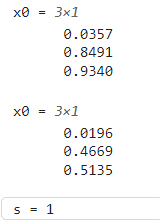
\includegraphics[width=0.32\linewidth]{img-147}
\caption*{\itshape $x_0$ alla creazione non è stocastico; dopo $x_0=x_0/\mathrm{sum}(x_0)$ la somma vale $1$.}
\end{figure}

Un semplice modello Simulink simula la stazionarietà della catena: un blocco
\emph{Unit Delay} (registro) restituisce in uscita il proprio ingresso con un passo di
ritardo (al primo passo l'ingresso è $x_0$); uno \emph{Scope} ne registra l'andamento, un
\emph{Display} mostra il valore corrente e un blocco \emph{Gain} moltiplica ad ogni passo
l'uscita del registro per la matrice $A$, generando il prossimo ingresso.

\mmacap[0.75]{img-148}{Modello Simulink della ricorsione $x(k+1)=A\,x(k)$}

Dopo circa cinque passi la catena converge ai valori mostrati dal \emph{Display}.

\mmacap[0.3]{img-149}{Andamento sullo Scope: convergenza della catena}

\paragraph{Calcolo in forma chiusa.}
Il risultato si dimostra rigorosamente cercando l'equilibrio stocastico $\Pi=A\Pi$. Se la
matrice $I-A$ è singolare esiste un vettore non nullo $\Pi$ che la soddisfa; per
determinarlo univocamente si costruisce il sistema formato dalle righe di $I-A$ e dalla
condizione di stato stocastico $\sum_i \Pi_i=1$. Risolvendo con \texttt{Solve} su
Mathematica si ottiene
\[
\Pi=\begin{bmatrix}\tfrac{75}{299}&\tfrac{114}{299}&\tfrac{110}{299}\end{bmatrix}^{\!\top}
\approx\begin{bmatrix}0{,}2508&0{,}3813&0{,}3679\end{bmatrix}^{\!\top},
\]
gli stessi valori mostrati dal \emph{Display} nella simulazione Simulink.

\mma[0.45]{img-153}

\subsection{Spanning tree}
Uno \emph{spanning tree} (albero ricoprente) è un albero che ha per nodi tutti i nodi del
grafo e un sottoinsieme dei suoi archi; essendo un albero è privo di cicli. Per il
\emph{Graph tree Markov chain theorem}, se dal grafo si estrae un albero i cui nodi foglia
sono gli elementi della catena e dal padre si raggiungono tutti i nodi foglia, allora
quell'albero è ricoprente.

\mmacap[0.4]{img-154}{Un possibile albero ricoprente della catena}


\end{document}
